\documentclass[12pt]{article}
\usepackage{graphicx}
\usepackage{amsmath}
\usepackage{amsfonts}
\usepackage{hyperref}

\begin{document}
\title{Tarea 2}
\author{Entrega: 16 de junio, 2026}
\date{}
\maketitle

En esta tarea, vamos a explorar la aplicación de MDPs a precios dinámicos, extendiendo el modelo visto en clase. Para los ejercicios en Python, puede copiar y modificar el  \href{https://colab.research.google.com/drive/1kfLv15ecpnXt09zmhkCLmLHK8DCtyHbe?usp=sharing}{notebook en Google Colab}.

\begin{enumerate}

\item Acá tenemos el gráfico ilustrando la política óptima obtenida en clase:
\begin{center}
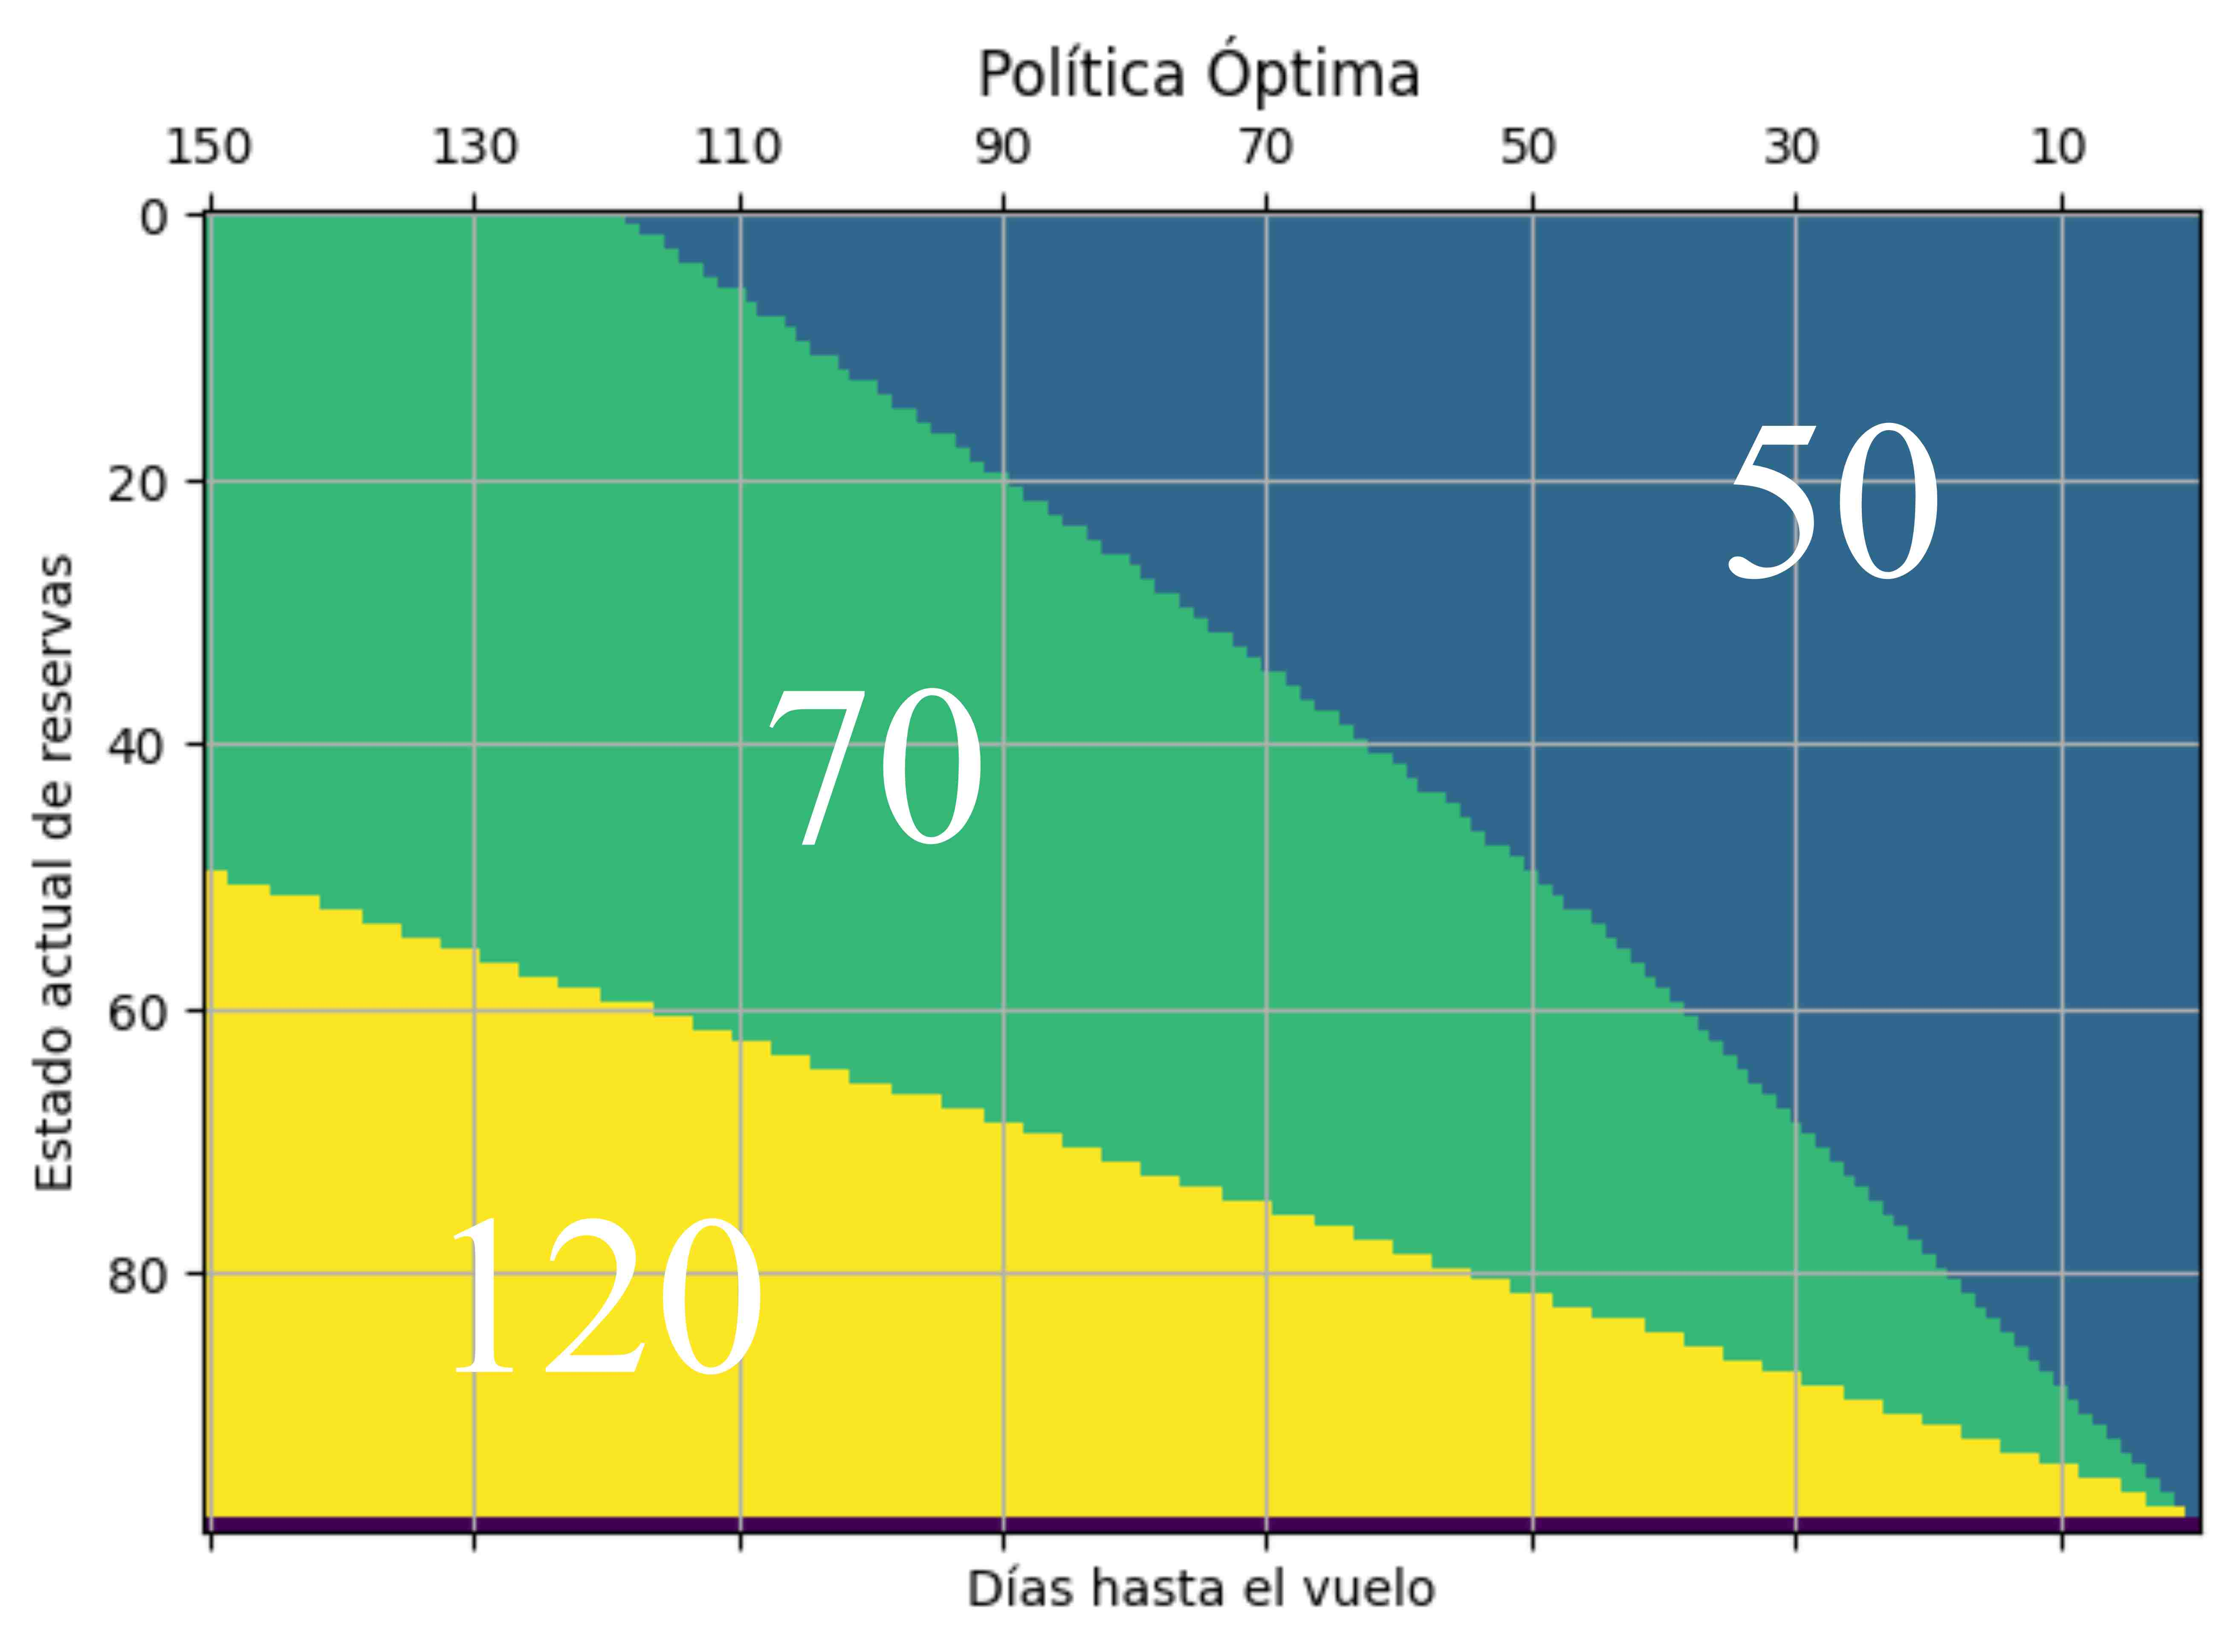
\includegraphics[width=0.6\textwidth]{../Images/Figures/DynamicPrices.jpg}    
\end{center}
\begin{enumerate}
\item ¿Qué ocurre con la política óptima de nuestro modelo teórico básico cuando faltan muy pocos días para el vuelo?
\item Consideremos el siguiente gráfico, que muestra el precio promedio de pasajes domésticos en EE.UU. (2012) en función de los días que restan para el despegue. Compare la política óptima calculada con nuestro modelo con los datos empíricos del gráfico de la industria aerocomercial. ¿Coinciden? Si observa discrepancias, ¿cómo explicaría la diferencia?
\begin{center}
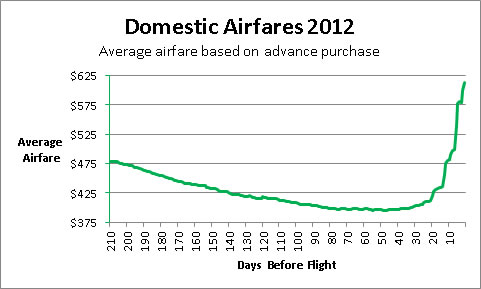
\includegraphics[width=0.55\textwidth]{../Images/Figures/2012-Domestic-Airfares.jpg}  
\end{center}
\end{enumerate}

\item Consideremos que el mercado está compuesto por dos segmentos de pasajeros con distintas distribuciones de disposición a pagar (valor máximo $m$):
\begin{itemize}
\item \textbf{Turistas:} $\mathbb{P}(m = 50) = 1/2$, $\mathbb{P}(m = 70) = 1/3$, $\mathbb{P}(m = 120) = 1/6$.
\item \textbf{Profesionales (Negocios):} $\mathbb{P}(m = 70) = 1/2$, $\mathbb{P}(m = 120) = 1/3$, $\mathbb{P}(m = 200) = 1/6$.
\end{itemize}
Suponga que a falta de $t$ días para el vuelo, la probabilidad de que el cliente potencial del día sea un Turista es $p_t$, y la probabilidad de que sea un Profesional es $1 - p_t$.

\begin{enumerate}
\item ¿Cómo espera que varíe la proporción $p_t$ a medida que se acerca la fecha del vuelo ($t \to 0$)? Justifique su razonamiento.
\item Especifique el modelo de MDP de horizonte finito bajo estas nuevas condiciones y escriba la ecuación de Bellman correspondiente.
\item Asumiendo que la dinámica temporal de la demanda sigue la curva $p_t = 1 - e^{-t/30}$:
\begin{itemize}
\item Modifique el código en Python para incorporar esta estructura de clientes variables en el tiempo.
\item Grafique la nueva política óptma y compárela con la del punto 1. ¿Logra esta extensión replicar cualitativamente el fenómeno observado en los datos reales del pasaje de EE.UU.? Desarrolle.
\end{itemize}
\end{enumerate}

\newpage
\item Vamos a extender el modelo incluyendo la posibilidad de gestionar cancelaciones y sobreventas:
\begin{itemize}
\item Se permite la sobreventa de pasajes. Pero al momento del despegue ($t=0$), si hay más pasajeros con pasaje en mano que asientos físicos en el avión, la aerolínea incurre en un costo de penalidad $L$ por cada pasajero desplazado.
\item Cada día, cada pasaje ya vendido tiene una probabilidad fija $\gamma$ de ser cancelado.
\end{itemize}
\begin{enumerate}
    \item Supongamos que, al cancelar su reserva, el cliente recibe un reembolso fijo de $\$50$, independiente del precio que haya pagado por el pasaje. Modele este problema como un MDP especificando sus componentes esenciales.
    
    \item Supongamos que el reembolso por cancelación corresponde al 80\% del precio real pagado por el pasaje. ¿Cómo debería cambiar el modelo de MDP? \textquestiondown Qu\'e impacto tiene esa nueva situaci\'on en la complejidad del modelo?
\end{enumerate}

\item En este ejercicio analizaremos la estructura de las fronteras de decisión y su impacto práctico en la toma de decisiones corporativas.

\begin{enumerate}
    \item En el gráfico del ejercicio 1 vemos que el modelo prescribe comenzar a ofrecer el precio mínimo de $\$50$ aproximadamente $120$ días antes del vuelo. A ese precio, el pasaje se vende con total certeza. Dado que el avión cuenta con una capacidad total de $100$ asientos, ¿por qué podría ser óptimo "rematar" asientos tan temprano en lugar de esperar, por ejemplo, hasta el día $100$ antes del despegue para bajar los precios? 
    
    \item La implementación base en Python elige la acción para cada estado mediante la función \textit{np.argmax}, seleccionando el primer índice/acción donde se alcanza el valor máximo (criterio de desempate por defecto), como podemos ver en la imagen del código de abajo:
    \begin{center}
        \makebox[\textwidth][c]{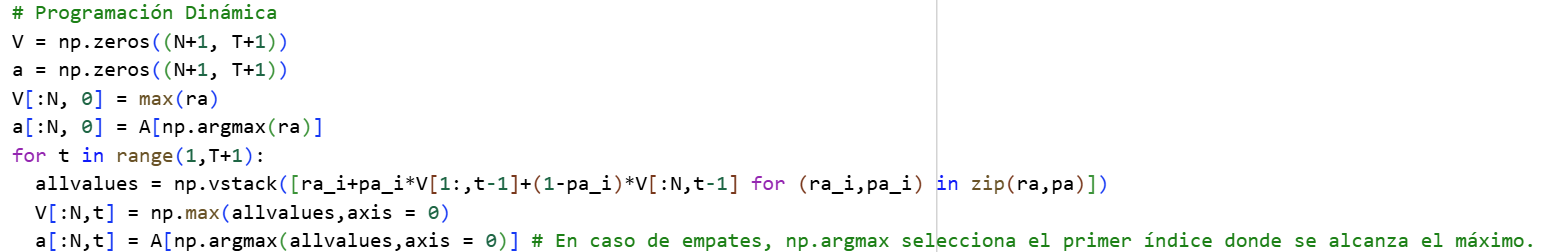
\includegraphics[width=1.2\textwidth]{../Images/Figures/dpprices.png}}
    \end{center}

    Modifique el código en Python removiendo los comentarios para invertir el orden de evaluación de las acciones (evaluando los precios de mayor a menor), como se indica en la imagen de abajo:
    \begin{center}
        \makebox[\textwidth][c]{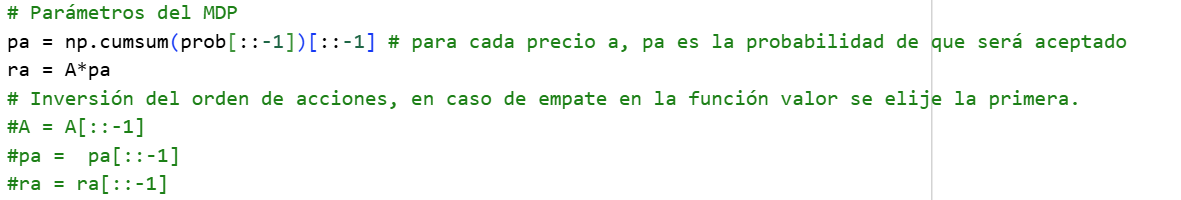
\includegraphics[width=1.2\textwidth]{../Images/Figures/invertactionorder.png}}
    \end{center}
    
    Con esta modificación realizada, resuelva:
    \begin{itemize}
        \item[\textbf{i)}] Grafique la nueva política óptima resultante.
        \item[\textbf{ii)}] ¿Cómo cambia la geometría de las fronteras de decisión? ¿Cambia la función de valor óptima $V(s,t)$? 
        \item[\textbf{iii)}] Desde una perspectiva de gestión de operaciones, ¿cuál de las dos políticas (fronteras curvas vs. fronteras lineales) considera que es más fácil de interpretar, auditar y comunicar al equipo de ventas o a los reguladores? Justifique.
    \end{itemize}
\end{enumerate}
\end{enumerate}
\end{document}